\documentclass[tikz, border=5pt]{standalone}

\usepackage[utf8]{inputenc}
\usepackage[upright]{fourier}

\usepackage{amsmath}
\usepackage{amssymb}
\usepackage{tikz}
\usetikzlibrary{matrix, fit, decorations.pathmorphing, arrows.meta}

\pgfdeclarelayer{bg}
\pgfdeclarelayer{fg}
\pgfsetlayers{bg,main,fg}

\begin{document}
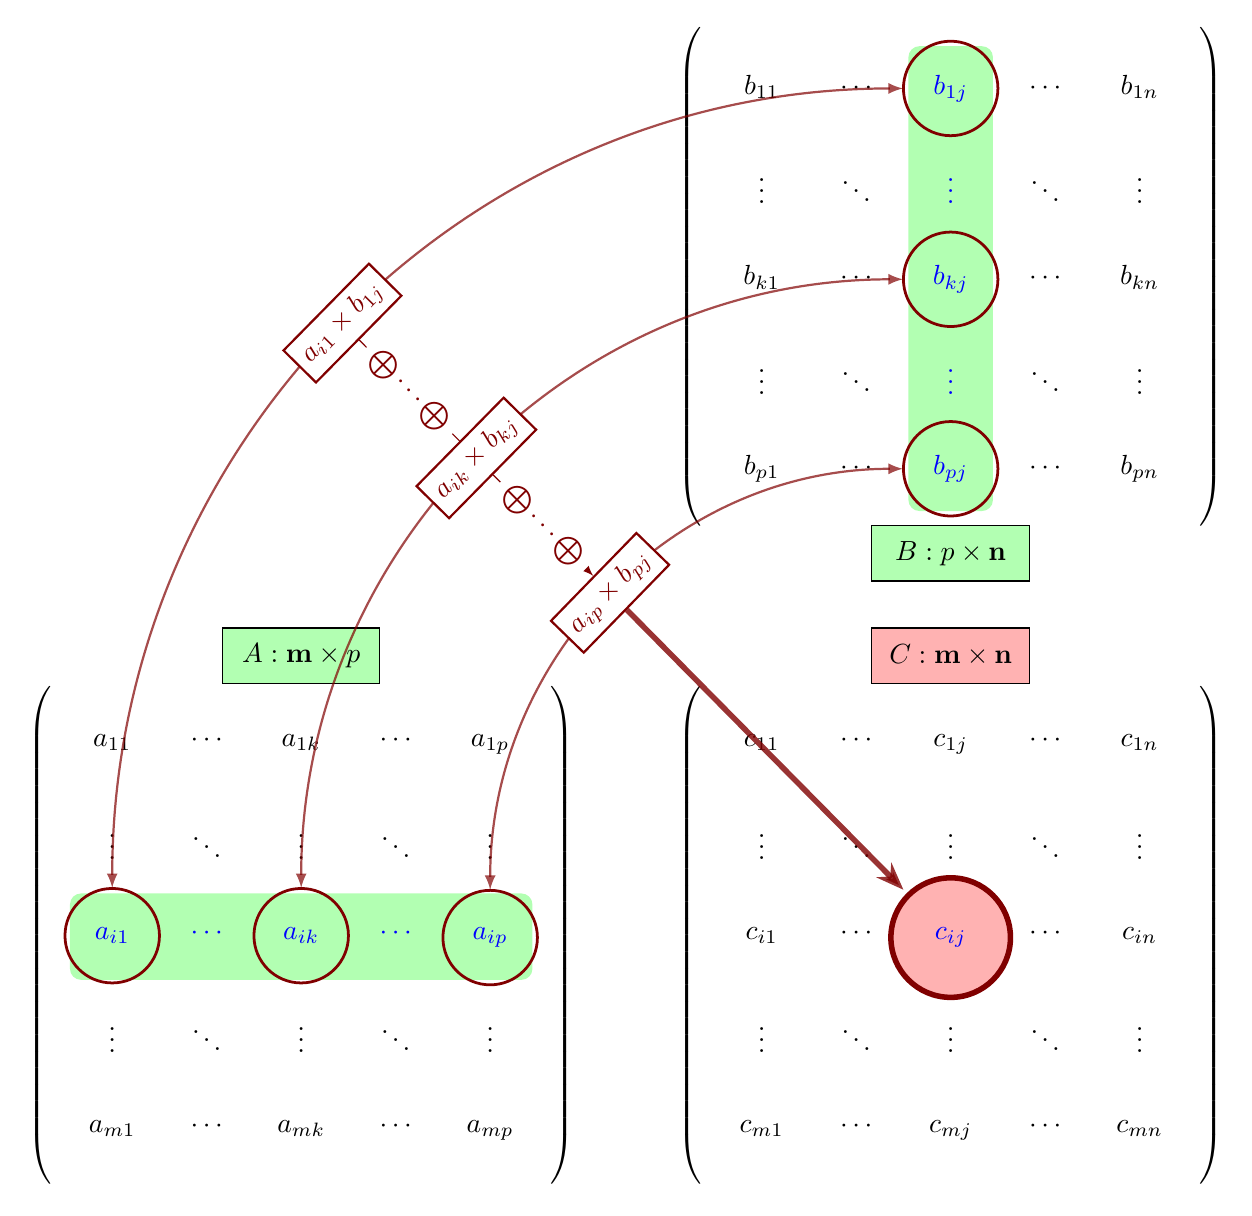
\begin{tikzpicture}[
% inner sep=0pt, outer sep=0pt
]

\tikzstyle{mat}=[matrix of math nodes, nodes={item}, left delimiter=(, right delimiter=), row 3 column 3/.style={nodes={blue}}]

% \tikzstyle{item}=[inner sep=0.3cm]
\tikzstyle{item}=[minimum size=1.2cm]

\tikzstyle{bblue}=[blue!50!black]
\tikzstyle{bred}=[red!50!black]

% C: mxn
\matrix (C) [mat] {
    c_{11} & \cdots & c_{1j} & \cdots &  c_{1n} \\
    \vdots & \ddots & \vdots & \ddots & \vdots \\
    c_{i1} & \cdots & c_{ij} & \cdots & c_{in} \\
    \vdots & \ddots & \vdots & \ddots & \vdots \\
    c_{m1} & \cdots & c_{mj} & \cdots & c_{mn} \\
};


% A: mxp
\matrix (A) [mat, anchor=east, xshift=-2cm, row 3/.style={nodes={blue}}] at (C.west) {
    a_{11} & \cdots & a_{1k} & \cdots & a_{1p} \\
    \vdots & \ddots & \vdots & \ddots & \vdots \\
    a_{i1} & \cdots & a_{ik} & \cdots & a_{ip} \\
    \vdots & \ddots & \vdots & \ddots & \vdots \\
    a_{m1} & \cdots & a_{mk} & \cdots & a_{mp} \\
};


% B: pxn
\matrix (B) [mat, anchor=south, yshift=2cm, column 3/.style={nodes={blue}}] at (C.north) {
    b_{11} & \cdots & b_{1j} & \cdots & b_{1n} \\
    \vdots & \ddots & \vdots & \ddots & \vdots \\
    b_{k1} & \cdots & b_{kj} & \cdots & b_{kn} \\
    \vdots & \ddots & \vdots & \ddots & \vdots \\
    b_{p1} & \cdots & b_{pj} & \cdots & b_{pn} \\
};


\tikzstyle{active}=[fill=green!30, rounded corners, inner sep=-2pt]
\begin{pgfonlayer}{bg}
    \node [active, fit=(A-3-1)(A-3-5)] {};
    \node [active, fit=(B-1-3)(B-5-3)] {};
    \node [active, fit=(C-3-3), draw=red!50!black, fill=red!30, line width=2pt, circle] {};
\end{pgfonlayer}{bg}

\tikzstyle{marked}=[item, draw=red!50!black, circle, line width=1pt]

% \foreach \co/\x in {1/1, 2/{...}, 3/k, 4/{...}, 5/p} {
\foreach \co/\x in {1/1, 3/k, 5/p} {
    \draw [latex-latex, opacity=0.7, thick, bred] (A-3-\co) to[out=90, in=180] node[sloped, midway, fill=white, draw, opacity=1] (mul\co) {$a_{i\x}\times b_{\x j}$} (B-\co-3);
    \node [marked] at (A-3-\co) {};
    \node [marked] at (B-\co-3) {};
}

\draw [bred,-latex] (mul1) to node [sloped, midway,fill=white] {$\bigoplus\cdots\bigoplus$} (mul3) to node[sloped,midway,fill=white] {$\bigoplus\cdots\bigoplus$} (mul5);

\draw [line width=2pt, opacity=0.8, bred, -{Stealth[length=10pt]}] (mul5) to (C-3-3);

\tikzstyle{matinfo}=[draw, inner sep=5pt, minimum width=2cm, minimum height=0.7cm]
\begin{pgfonlayer}{bg}
\node [matinfo, fill=green!30, yshift=10pt] at (A.north) {$A: \mathbf{m} \times p$};
\node [matinfo, fill=green!30, yshift=-10pt] at (B.south) {$B: p \times \mathbf{n}$};
\node [matinfo, fill=red!30, yshift=10pt] at (C.north) {$C: \mathbf{m \times n}$};
\end{pgfonlayer}


\end{tikzpicture}
\end{document}
